
After representing the data in functional form, and preprocessing it to quantify and
reduce its variability, it may be interesting to study the relationship between
various functional variables. As in Multivariate Statistics and Machine Learning,
\acs{FDA} will deal with the regression and classification problems, but in the case
where some of the data are of a functional nature.


In \textit{classification}, or more precisely supervised classification, the category or
population to which an observation belongs is studied, using a set of data whose
category is known. For example, predicting the climate type of a region from
its temperature curves is a functional classification problem.

In \textit{regression} is studied the existing relation between two or several
random variables. Instead of predicting a class label, as in classification,
regression models are created to predict another variable, called dependent
variable or response, from one or more known variables. In the case of
functional prediction we must make a distinction that does not appear in
classical statistics between two cases, when the response to predict is an
scalar quantity or is also a functional datum. For instance, the prediction of
the total precipitation of a region from its temperature curves is a regression
problem with scalar response, as opposed to the case with functional response,
in which is predicted the precipitation curves from the temperatures.
Among the models most used for these two problems can be found the nearest
neighbors estimators.

\newacronym{NN}{NN}{Nearest Neighbors}


The \ac{NN} estimators are a family of methods widely
used in Statistics and Machine Learning, in problems of classification or
regression, among others. These estimators are based on the idea of
neighborhood, using the notion of distance, so that it is made a local
estimation of the density of the data.
Although in their classic version they are used with sets of vectors,
their ideas work in the same way in general metric
spaces \cite{baillo2010}, as the functional ones we consider in this work.

Let $(\mathcal{F}, d)$ be a metric space and
$(f_i, {Y}_i)_{i \le i \le n}$ a training set with their
respective labels or responses.
To estimate a datum $x$, either for classification or prediction of its
response, firstly, it will be necessary to find the elements of the training set
closest to this datum, which will form its neighborhood, denoted as $k(x)$.

\newacronym{KNN}{KNN}{K-Nearest Neighbors}

There are two variants of these methods. In the first one, consisting of
\ac{KNN} estimators, it is taken as neighborhood the $k$ closest
elements to $x$, i. e., if the training pairs are re-indexed as
$(f_{(i)}, Y_{(i)}) \, 1\le i\le n$ so that the
$f_{(i)}$'s are re-arranged in increasing distance from $x$,
$d(x, f_{(1)}) \le d(x, f_{(2)}) \le \dots \le d(x, f_{(n)})$,
 then $k(x) = \{f_{(i)} \, : \, 1 \le i \le i\le k\}$.

\begin{figure}[Neighborhoods using distance $\mathbb{L}^\infty$]{FIG:NNSEARCH}{neighborhoods using distance $\mathbb{L}^\infty$}
	\subfigure[SBFIG:NNSEARCH1]{K-nearest neighbors}{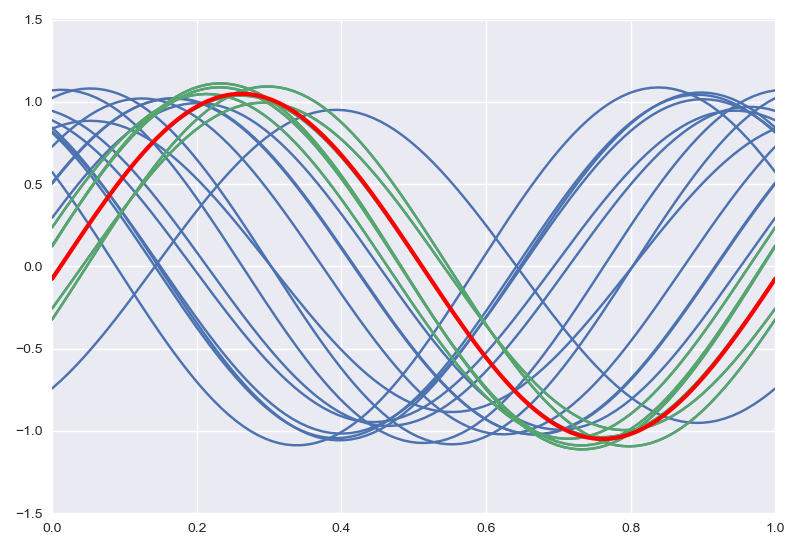
\includegraphics[width=7cm]{k-search}} \quad
	\subfigure[SBFIG:NNSEARCH2]{Radius-nearest neighbors}{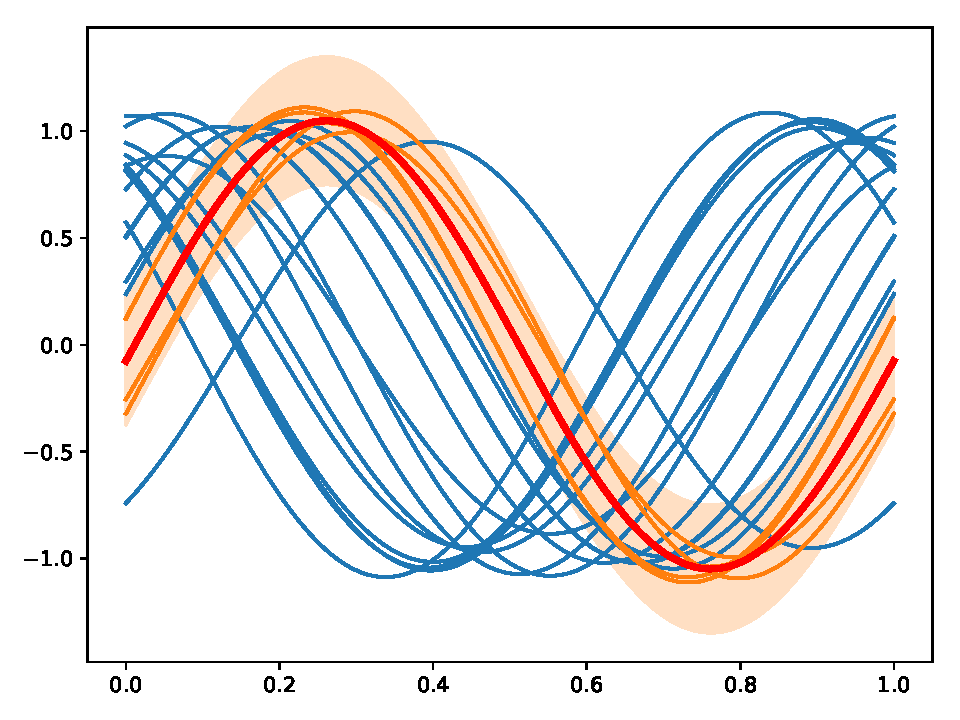
\includegraphics[width=7cm]{radius-search}}
\end{figure}

In the second variant, less used in practice, consisting of the radius neighbors
estimators, the neighborhood contains the samples $f_i$ in the ball of
radius $r$ centered in $x$, i.e.
$k(x) = \{ f_i : d(f_i , x) \le r\}$. For instance, if we
use the distance $\mathbb{L}^\infty$, we may visualize $k(x)$ as the set of all
functions within a band  of radius $r$ around $x$.
In the figure \ref{FIG:NNSEARCH} there are shown the neighborhoods with these two different
approaches.

In practice, for the construction of the neighborhoods, the simplest solution is
 to perform a linear search, calculating the distances between $x$ and all the
 elements of the training set.
The naïve approach of the linear search may be improve using data structures
based on spatial indexes, such as ball trees \cite{Kumar2008}. However, the best
nearest-neighbors data structure for a given application will depend on the
dimensionality, size, and underlying structure of the data.
